\chapter[Patient journey - 1]{Patient journey based on first-time prescriptions}
After the preliminary analysis and deciding the main focus area, there are enough information to begin reconstructing the \textbf{patient journey}. The goal of this process is to highlight changes in \textit{prescription patterns for chronic diseases}, starting from the medical history of patients.

An objective definition of patient journey can be created using the following guidelines:
\begin{enumerate}
	\item Patients with \textbf{complete medical history} for a fixed amount of years;
	\item Records with patient, prescribing GP, diagnosis and prescription on the \textbf{same date};
	\item Only \textbf{first-time }diagnoses and prescriptions considered.
\end{enumerate}

The imposed criteria is very strict: taking diagnoses and prescriptions on the same day means removing \textit{all prescriptions} following the first diagnosis. In other words, all the instances of patients coming back to their GP to renew a prescription for a chronic disease have been deleted.

This can be useful to extract a cohort of patients beginning their treatment, and analyse the variations of first-time prescriptions. It's important to notice that not all doctors may have patients with a new chronic illness.

\section{Imposed criteria}
Aside from the completeness and correctness of the data, there are more restrictions to maintain the consistency:
\begin{itemize}
	\item The prescribing general practitioner mustn't change in the time range;
	\item The patient mustn't be deceased;
	\item There must be a sanitary convention;
	\item The general practitioner must be active.
\end{itemize}

All those constraints can be checked using the related fields in the database: \textit{pa\_drevoca} for interruption of the relationship, \textit{decesso} for death and \textit{pa\_convenzione} for the sanitary convention.

The table \textit{users} contains all the IDs of active general practitioners, so joining it with other tables is enough to remove all the rows with an inactive GP. Data is up to date, but since the patient journey will include 2018 (the focus is on the most recent information) there is no need to check for active GPs in the previous years.

The biggest risk is again the \textbf{loss of information}: the impact of data cleansing is heavy, and the obtained results might not give an insightful prospective.

\section{Initial data cleaning}
An initial data cleaning has been made on the whole database to have a first understanding of the potential information loss.

In this case, having such a big amount of tuples is useful: it's possible to remove a considerable percentage of them without losing generality and still having numerous samples.

Information on the general loss is already available thanks to the specific analysis on each single field, so the shown data cleaning will only consider patients and GPs.

The active general practitioners are \textbf{432}: this result has been retrieved counting the different IDs in \textit{users} (438) and removing the ones that weren't present in \textit{nos\_002} (6).

The following \textit{pie chart} illustrates the data loss on patients according to the criteria defined in the previous section.
\begin{figure}[h]
	\centering
	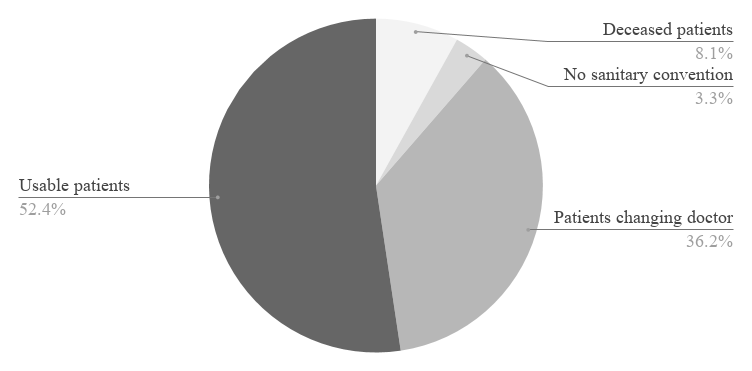
\includegraphics[scale=0.6]{immagini/pie0018.png}
\end{figure}

About half of patients is going to be lost, due to not respecting the consistency criteria. Starting from a million of records, concrete results are still obtainable.

\section{First approach}
The first approach consists in testing with an \textbf{arbitrary range constraint}: all dates must fall in the span between 2010 and 2018.

The analysis has pure research purposes, to understand the impact of a cut of the dataset in terms of information loss. All the previously introduced criteria must be considered as well, so there must be a continuous doctor-patient relationship between active GPs and non-deceased patients with sanitary conventions.

The outcome is a patient journey table containing data from 2000 to 2018, with a total amount of \textbf{144.618} tuples: this means that there are roughly 150k of first-time diagnosis and prescriptions to patients. 

\subsection{Results breakdown}
Seeing that the starting tables had number of rows in the order of millions, some deeper analysis is necessary to figure out the causes of this huge loss.

The 144.618 complete tuples are composed by:
\begin{itemize}
	\item 27.733 patients;
	\item 422 general practitioners;
	\item 1.381 unique diagnoses;
	\item 904 unique prescriptions.
\end{itemize}

Further causes for those low values can be found counting how many dates would not fall in the considered range. The percentage of records with date earlier than 2010 in each table is:
\begin{itemize}
	\item Patients: 75\%;
	\item Diagnosis: 54,6\%;
	\item Prescriptions: 44,7\%.
\end{itemize}

There is an enormous loss on patients: the possible reason might be that most patients started treatment earlier than 2010, plus diagnosis and relative prescription are in different dates.

8 years is a too wide range to obtain a consistent patient journey, and such information loss isn't negligible: the conclusion of the first approach is that introducing time boundaries is something which needs an accurate control, to avoid missing out most of the data.

\newpage
\section{Second approach}
Since just removing according to the date is an abrupt approach, it's necessary to tune parameters and introduce more detailed constraint, to have a bigger amount of information.

The focus is on the number of prescriptions: given a small range of years, only patients with at least one new prescription are going to be considered. All the previous criteria must be respected, so there must be a continuous doctor-patient relationship between active GPs and non-deceased patients with sanitary conventions.

This methodology allows cluster sampling without having to remove half of the dates: criteria based on the number of prescriptions creates another patient cohort which can be used to accurately select rows from the other tables.

The proposed time range is 2016-2018: pharmaceutical companies generally use the last two years of sales, so picking the last three years gives additional information without compromising the consistency of data.

The outcome is a patient journey consisting of 1.465.005 tuples: almost 10 times the previous result. This leads to two important statements:
\begin{enumerate}
	\item The time range is appropriate, since the number is large enough to make analysis without loss of generality;
	\item The new imposed criterion gives more consistent data and the possibility to build time series.
\end{enumerate}

More cleaning is required to link diagnoses and prescriptions, since there is not a 1:1 correspondence: multiple diagnosis and prescriptions may be associated to the same date. This can be done using a lookup table.

\subsection{Results breakdown}
The 1.665.005 complete tuples are composed by:
\begin{itemize}
	\item 230.381 patients;
	\item 422 general practitioners;
	\item 1.381 unique diagnoses;
	\item 904 unique prescriptions.
\end{itemize}

Only 7\% of the total prescription has been taken in consideration, yet a million and half is still a satisfying amount.

\section{Results comparison}
Comparing the two patient journey outcomes through graphs is a good way to visualize changes and improvements.

\subsection{Changes in data composition}
% todo

\subsection{Improvement on patients information loss}
% todo
A pie chart for data loss on patients in the range 2016-2018 has been made to compare with the previous one.

\begin{figure}[h]
	\centering
	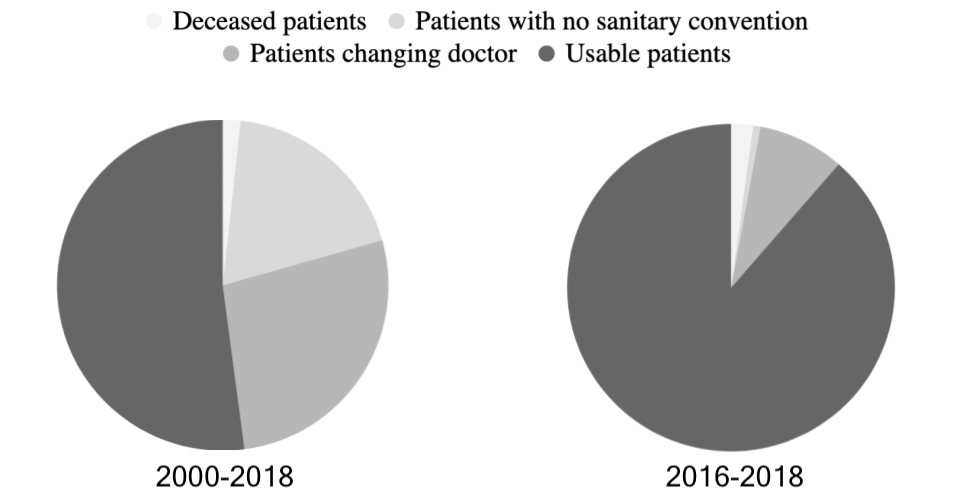
\includegraphics[scale=0.5]{immagini/pies.png}
\end{figure}

It's easy to see that the number of usable patients has noticeably increased: using a smaller time span reduces the chances of death and change of GP.

\subsection{Funnel graph of patients}
A funnel graph is useful to see how imposing every restriction made the patients number decrease: starting from a million, in the end there only is about $\nicefrac{1}{4}$ of it.







